\newpage
\section{Dynamic programming problems} \label{problems}
% ------------------------------------------------------------------------------------------------
\subsection{Problems classification}
\subsubsection{Definitions}\ul
\item \textbf{Alphabets:} the alphabet represent an enumeration of the possible values. Their size helps determining how many bits are required in the implementation to store the values. Alphabets must be defined for input, wavefront, cost and backtrack.
\item \textbf{Dimensions:} let $n$ the size of the input and $d$ the dimension of the underlying matrix.
\item \textbf{Matrices:} we refer indifferently by the matrix or the matrices to all the intermediate cost- and backtrack-related informations that are necessary to solve the dynamic programming problem of interest. Matrices elements are usually denoted by $M_{(i,j)}$ ($i^{\rm th}$ line , $j^{\rm th}$ column).
\item \textbf{Computation block:} this is a part of the DP matrix (cost and or backtrack) that we want to compute. A block might be either a sub-matrix (rectangular) or a parallelogram, possibly cropped at its parent matrix boundaries.
\item \textbf{Wavefront:} the wavefront consists of all the data necessary to reconstruct a computation block of the DP matrix. It might include some previous lines/columns/diagonals as well as line-/column-/diagonal-wise aggregations (min, max, sum, ...).
\item \textbf{Delay:} we call delay the maximum distance between an element and its dependencies along column and lines (ex: recurrence $M_{(i,j)}=f\big(M_{(i-1,j)}, M_{(i-2,j-1)}\big)$ has delay 3).
\ule

\subsubsection{Litterature classification}
In the literature, dynamic programming problems are classified according to two criteria:\ul
\item \textbf{Monadic/polyadic:} a problem is monadic when only one of the previously computed term appears in the right hand-side of the recurrence formula (ex: Smith-Waterman). When two or more terms appear, the problem is polyadic (ex: Fibonacci, $F_n = F_{n-1} + F_{n-2}$).
When a problem is polyadic with index $p$, it also means that its backtracking forms a $p$-ary tree (where each node has at most $p$ children).

\item \textbf{Serial/non-serial:} a problem is serial ($s=0$) when the solutions depends on a fixed number of previous solutions (ex: Fibonacci), otherwise it is said to be non-serial ($s\ge 1$), as the number of dependencies grows with the size of the subproblem. That is computing an element of the matrix would require $O(n^s)$.  (ex: Smith-Waterman with arbitrary gap is $s=1$; we can usually infer $s$ from the number of bound variables in the recurrence formula)
	\[M_{(i,j)}=\max\left\{\begin{array}{l} ... \\ M_{(i,j-1)}\\ \max\limits_{i<k<j} [ M_{(i,k)}+M_{(k+1,j)} ] \end{array}\right. \]
\ule

Note that the algorithmic complexity of a problem is exactly $O\big(n^{d+s}\big)$.

\subsubsection{Calculus simplifications}
In some special case, it is possible to transform a non-serial problem into a serial problem, if we can embed the non-serial term into an additional aggregation matrix. For example:
	\[M_{(i,j)}=\max\left\{\begin{array}{l} \max\limits_{k<i} M_{(k,j)}
	\\ \sum\limits_{k<i, l<j}M_{(k,l)} \end{array}\right.
	\implies M_{(i,j)}=\max\left\{\begin{array}{l} C_{(k,j)} \\ A_{(i-1,j-1)} \end{array}\right.\]
Where the matrix $C$ stores the maximum along the column and matrix $A$ stores the sum of the array of the previous elements. Both can be easily computed with an additional recurrence:
	\[\begin{array}{rcl} C_{(i,j)}&=&\max(C_{(i-1,j)}, M_{(i,j)}) \\
	A_{(i,j)}&=&A_{(i-1,j)}+A_{(i,j-1)}-A_{(i-1,j-1)}+M_{(i,j)}\end{array}\]

Although this simplification removes some non-serial dependencies at the cost of extra storage in the wavefront, it is not sufficient to transform all non-serial monadic problems into serial problems (ex: this does not apply to Smith-Waterman with arbitrary gap cost).

% ------------------------------------------------------------------------------------------------
\subsection{Problems of interest}
We usually focus on problem that have an underlying bi-dimensional matrix ($d=2$) because they can be parallelized (as opposed to be serial if $d=1$) and can solve large problems (of size $n$). Problems of higher matrix dimensionality ($d\ge3$) require substantial memory which severely impacts their scalability. Also we tend to limit algorithmic complexity of the problems as from $O(n^4)$ on, running time becomes a severely limiting factor.

We describe problems structures: inputs, cost matrices and backtracking matrix. These all have an alphabet (that must be bounded in terms of bit-size). Unless otherwise specified, we adopt the following conventions:\ul
\item Vectors of size $n$ are indexed from 0 to $n-1$, matrices follow the same convention ($M_{(m,n)}$ is indexed from $(0,0)$ to $(m-1,n-1)$)
\item Matrices dimensions are implicitly specified by number of indices and their number of elements is usually the same as the input length (possibly with 1 extra row/column).
\item Number are all unsigned integers
\item Problem dimension is $m,n$ (or $n$) indices $i,j$ ranges are respectively $0\le i<m$, $0\le j<n$.
\item Unless otherwise specified, the recurrence applies to all non-initialized matrix elements.
\ule
We describe the problem processing in terms of both initialization and recurrences.

Although not necessary to understand the project, the description of some of the most common dynamic programming problem is relevant to capture the essence of the dynamic programming processes and be able to compare and search for similarities among problems. Would the reader be familiar with dynamic programming, he could immediately jump to the next section.

A tighter analysis on the alphabet and intermediate results size is done because FPGA was also considered as a possible execution platform.\footnote{Initially, the project envisioned a collaboration with \href{mailto:nithin.george@epfl.ch}{Nithin George}, a PhD student at Processor Laboratory (LAP), EPFL. Unfortunately, at the time of writing, progress in this direction is not sufficient to be covered in this report. However, FPGA is considered as a future deployment platform for a particular class of problems.}

% ------------------------------------------------------------------------------------------------
% Recurrence visualization helpers
\newcommand\Cd[3][0,-1]{\put(#2){\put(.5,.5){\circle*{.3}}\put(.5,.5){\linethickness{1.5pt}\vector(#1){#3}}}} % dependency [dx,dy]{x,y}{len}
\def\Cg#1{\put(#1){\color{lightgray}\put(0,0){\polygon*(0,0)(0,1)(1,1)(1,0)}}} % grayed cell (not to store
\def\Cz#1{\put(#1){\put(0,.35){\parbox{1\unitlength}{\centering\bf 0}}}} % zero-init cell
\def\Cm{\put(6.5,4.5){\circle*{.4}}\multiput(0,0)(1,0){9}{\line(0,1){8}}\multiput(0,0)(0,1){9}{\line(1,0){8}}} % matrix base
\def\Cfl#1{#1{0,6}#1{0,5}#1{1,5}#1{0,4}#1{1,4}#1{2,4}#1{0,3}#1{1,3}#1{2,3}#1{3,3}#1{0,2}#1{1,2}#1{2,2}#1{3,2}#1{4,2}
	#1{0,1}#1{1,1}#1{2,1}#1{3,1}#1{4,1}#1{5,1}#1{0,0}#1{1,0}#1{2,0}#1{3,0}#1{4,0}#1{5,0}#1{6,0}} % triangular lower (function)
\def\Cfd#1{#1{0,7}#1{1,6}#1{2,5}#1{3,4}#1{4,3}#1{5,2}#1{6,1}#1{7,0}} % main diagonal
\def\Cfdu#1{#1{7,1}#1{6,2}#1{5,3}#1{4,4}#1{3,5}#1{2,6}#1{1,7}} % upper diagonal

%\def\Cmlong{\put(6.5,4.5){\circle*{.4}}\multiput(0,0)(1,0){16}{\line(0,1){8}}\multiput(0,0)(0,1){9}{\line(1,0){15}}} % matrix base
%\def\Cfu#1{#1{8,7}#1{9,7}#1{10,7}#1{11,7}#1{12,7}#1{13,7}#1{14,7}#1{9,6}#1{10,6}#1{11,6}#1{12,6}#1{13,6}#1{14,6}#1{10,5}#1{11,5}#1{12,5}#1{13,5}#1{14,5}#1{11,4}#1{12,4}#1{13,4}#1{14,4}#1{12,3}#1{13,3}#1{14,3}#1{13,2}#1{14,2}#1{14,1}} % triangular upper (function)

% ----------------------------------------------
\newpage
\subsubsection{Smith-Waterman (simple)}\label{sswat}\ol
\item Problem: matching two strings $S$, $T$ with $|S|=m, |T|=n$.
\item Matrices: $M_{(m+1) \times (n+1)}, B_{(m+1) \times (n+1)}$
\item Alphabets:\ul
	\item Input: $\Sigma(S)=\Sigma(T)=\{a,c,g,t\}$.
	\item Cost matrix: $\Sigma(M) = [0..z], z=\max({\rm cost(\_,\_)}) \cdot \min(m,n)$
	\item Backtrack matrix: $\Sigma(B)=\{stop,W,N,NW\}$
	\ule
\item Initialization:\ul
	\item Cost matrix: $M_{(i,0)}=M_{(0,j)}=0$.
	\item Backtrack matrix: $B_{(i,0)}=B_{(0,j)}=stop$.
	\ule
\item Recurrence: \[M_{(i,j)}=\max\left\{\begin{array}{l|l}
		0 & stop\\
		M_{(i-1,j-1)}+{\rm cost}(S(i-1),T(j-1)) & NW\\
		M_{(i-1,j)}-d & N\\
		M_{(i,j-1)}-d & W
	\end{array}\right\}=B_{(i,j)} \]

\item Backtracking: starts from the cell $M_{(m,n)}$ and stops at the first cell containing a $0$.
\item Visualization: by convention, we put the longest string vertically ($m\ge n$):
\begin{center}\setlength{\unitlength}{.6cm}\begin{picture}(8,9)
	\put(-.5,7.5){S}\put(-.35,7.4){\linethickness{1pt}\vector(0,-1){2}}
	\put(.2,8.2){T}\put(.8,8.4){\linethickness{1pt}\vector(1,0){2}}
	\Cz{0,0}\Cz{0,1}\Cz{0,2}\Cz{0,3}\Cz{0,4}\Cz{0,5}\Cz{0,6}\Cz{0,7}
	\Cz{1,7}\Cz{2,7}\Cz{3,7}\Cz{4,7}\Cz{5,7}\Cz{6,7}\Cz{7,7}
	\Cd{6,5}{0.8}
	\Cd[1,0]{5,4}{0.8}
	\Cd[1,-1]{5,5}{0.8}
\Cm\end{picture}\end{center}

\item Optimizations:\ul
	\item In serial (monadic) problems we can avoid building the matrix $M$ by only maintaining the 3 last diagonals in memory (one for the diagonal element, one for horizontal/vertical, and one being built). This construction extends easily to polyadic problems where we need to maintain $k+2$ diagonals in memory where $k$ is the maximum backward lookup.
	\item Since first line and column of the matrix (corresponding to a matching with one string being empty) are zeroed, their initialization might be omitted, but this would implies more involved initialization and computations, which is cumbersome.
	\item Padding: since to fill the $i^{\rm th}$ row we refer to the $(i-1)^{\rm th}$ character of string $S$, we could prepend to both $S$ and $T$ an unused character, so that matrix and input lines are aligned. Hence valid input indices would become $S[1 \cdots m]$ and $T[1 \cdots n]$.
	\ule
\ole

% ----------------------------------------------
\newpage
\subsubsection{Smith-Waterman with affine gap extension cost}\ol

\item Problem: matching two strings $S$, $T$ with $|S|=m, |T|=n$.
\item Matrices: $M_{(m+1) \times (n+1)}, E_{(m+1) \times (n+1)}, F_{(m+1) \times (n+1)}, B_{(m+1) \times (n+1)}$
\item Alphabets:\ul
	\item Input: $\Sigma(S)=\Sigma(T)=\{a,c,g,t\}$.
	\item Cost matrices: $\Sigma(M) = \Sigma(E) = \Sigma(F) = [0..z], z=\max({\rm cost(\_,\_)}) \cdot \min(m,n)$
	\item Backtrack matrix: $\Sigma(B)=\{stop,W,N,NW\}$
	\ule
\item Initialization:\ul
	\item No gap cost matrix: $M_{(i,0)}=M_{(0,j)}=0$.
	\item T-gap extension cost matrix: $E_{(i,0)}= 0$ \textit{<<eat S chars only>>}
	\item S-gap extension cost matrix: $F_{(0,j)}= 0$
	\item Backtrack matrix: $B_{(i,0)}=B_{(0,j)}=stop$.
	\ule
\item Recurrence for the cost matrices:
\[\begin{array}{rcl}
M_{(i,j)}&=&\max\left\{\begin{array}{l|l}
	0 & stop\\
	M_{(i-1,j-1)}+{\rm cost}(S(i-1),T(j-1)) & NW\\
	E_{(i,j)} & N\\
	F_{(i,j)} & W
\end{array}\right\}=B_{(i,j)}\\
\\
E_{(i,j)}&=&\max\left\{\begin{array}{l|l}
	M_{(i, j-1)} - \alpha & NW\\
	E_{(i,j-1)} - \beta & N\\
\end{array}\right\}=B_{(i,j)}\\
\\
F_{(i,j)}&=&\max\left\{\begin{array}{l|l}
	M_{(i-1,j)} - \alpha & NW\\
	F_{(i-1,j)} - \beta & W\\
\end{array}\right\}=B_{(i,j)}
\end{array}\]

That can be written alternatively as:
\[M_{(i,j)}=\max\left\{\begin{array}{l|l}
	0 & stop\\
	M_{(i-1,j-1)}+{\rm cost}(S(i-1),T(j-1)) & NW\\
	\max_{1 \le k \le j-1} M_{(i,k)} - \alpha - (j-1-k) \cdot \beta & N\\
	\max_{1 \le k \le i-1} M_{(k,j)} - \alpha - (i-1-k) \cdot \beta & W\\
\end{array}\right\}=B_{(i,j)} \]

Although the latter notation seems more explicit, it introduces non-serial dependencies that the former set of recurrences is free of. So we need to implement the former rules whose kernel is 
\[ [M;E;F]_{(i,j)} = f_{\rm kernel} ( [M;E]_{(i,j-1)}, [M;F]_{(i-1,j)}, M_{(i-1,j-1)} ) \]
Notice that this recurrence is very similar to \nameref{sswat} except that we propagate 3 values ($M,E,F$) instead of a single one ($M$). Also notice that it is possible to propagate $E$ and $F$ inside a resp. horizontal and vertical wavefront.

\item Backtracking, visualization and optimizations are the same as in \nameref{sswat}
\ole

% ----------------------------------------------
\newpage
\subsubsection{Smith-Waterman with arbitrary gap cost}\label{aswat}\ol
\item Problem: matching two strings $S$, $T$ with $|S|=m, |T|=n$ with an arbitrary gap function $g(x)\ge 0$ where $x$ is the size of the gap. Without loss of generality, let $m\ge n$ (swap inputs if necessary). Example penalty function could be\footnote{Intuition: long gaps penalize less, at some point, one large gap is better than matching with smaller gaps.} $g(x)=m-x$.
\item Matrices: $M_{(m+1) \times (n+1)}, B_{(m+1) \times (n+1)}$
\item Alphabets:\ul
	\item Input: $\Sigma(S)=\Sigma(T)=\{a,c,g,t\}$.
	\item Cost matrix: $\Sigma(M) = [0..z], z=\max({\rm cost(\_,\_)}) \cdot \min(m,n)$
	\item Backtrack matrix: $\Sigma(B)=\{stop,NW,N_{\{0..m\}},W_{\{0..n\}}\}$
	\ule

\item Initialization:\ul
	\item Match cost matrix: $M_{(i,0)}=M_{(0,j)}=0$.
	\item Backtrack matrix: $B_{(i,0)}=B_{(0,j)}=stop$.
	\ule

\item Recurrence: \[M_{(i,j)}=\max\left\{\begin{array}{l|l}
	0 & stop\\
	M_{(i-1,j-1)}+{\rm cost}(S(i-1),T(j-1)) & NW\\
	\max_{1 \le k \le j-1} M_{(i,j-k)} - g(k) & N_k\\
	\max_{1 \le k \le i-1} M_{(i-k,j)} - g(k) & W_k\\
\end{array}\right\}=B_{(i,j)} \]

\item Backtracking: similar to \nameref{sswat} except that you can jump of $k$ cells along the rows or along the columns.
\item Visualization:
	\begin{center}\setlength{\unitlength}{.6cm}\begin{picture}(8,9)
		\put(-.5,7.5){S}\put(-.35,7.4){\linethickness{1pt}\vector(0,-1){2}}
		\put(.2,8.2){T}\put(.8,8.4){\linethickness{1pt}\vector(1,0){2}}
	\Cz{0,0}\Cz{0,1}\Cz{0,2}\Cz{0,3}\Cz{0,4}\Cz{0,5}\Cz{0,6}\Cz{0,7}
	\Cz{1,7}\Cz{2,7}\Cz{3,7}\Cz{4,7}\Cz{5,7}\Cz{6,7}\Cz{7,7}
		\Cd[0,-1]{6,7}{2.8}\Cd[0,-1]{6,6}{1.8}\Cd{6,5}{0.8}
		\Cd[1,0]{0,4}{5.8}\Cd[1,0]{1,4}{4.8}\Cd[1,0]{2,4}{3.8}\Cd[1,0]{3,4}{2.8}\Cd[1,0]{4,4}{1.8}\Cd[1,0]{5,4}{0.8}
		\Cd[1,-1]{5,5}{0.8}
	\Cm\end{picture}\end{center}

\item Optimizations: The dependencies here are non-serial, there is no optimization that we can apply out of the box here. In general, this problem has an $O(n^3)$ complexity (whereas simple and affine gap variants are $O(n^2)$).
\ole

% ----------------------------------------------
\newpage
\subsubsection{Convex polygon triangulation}\ol
\item Problem: triangulating a polygon of $n$ vertices with least total cost for added edges. We denote the cost of adding an edge between the  pair of edges $i,j$ by $S_{(i,j)}$, Where $S_{n \times n}$ is a symmetric matrix (can be stored as a triangular matrix with 0 diagonal that can be omitted), hence $|S|=\tfrac{n(n-1)}{2}=N$.
\item Matrices: $M_{(n+1)\times (n+1)}, B_{(n+1)\times (n+1)}$ \textit{indices denote <<first vertex, last vertex>>}.\\ Upper triangular matrices including main diagonal. Note that the vertex $n$ is the same as the vertex $0$ due to the cyclic nature of the problem.
\item Alphabets:\ul
	\item Input: $\Sigma(S_{(i,j)})=\{0..m\}$ with $m=\max_{i,j} S_{(i,j)}$ determined at runtime\footnote{We need to have statistics about $S$, this is where dynamic compilation might play a role}.
	\item Cost matrix: $\Sigma(M)=\{0..z\}$ with $z = m \cdot (n-2)$ (a triangulation of a polygon of $n$ edges adds at most $n-2$ edges).
	\item Backtrack matrix: $\Sigma(B)=\{stop, 0..n\}$ (index of intermediate edge)
	\ule
\item Initialization: $M_{(i,i)}=M_{(i,i+1)}=0, B_{(i,i)}=B_{(i,i+1)}=stop \quad\forall i$
\item Recurrence: \[M_{(i,j)}=\left\{ S(i,j) + \max_{i<k<j}M_{(i,k)}+M_{(k,j)} \,\,\rule[-.75em]{.5pt}{2em}\,\,  k \right\} = B_{(i,j)} \]
	Intuition: triangulate the partial polygon $(i,..j)$ recursively. For the last triangle of the polygon consider 3 cases:\ul
	\item Given 2 triangulations $(1..k)$ and $(k..n)$, we close the polygon with $\bigtriangleup(1,k,n)$
	\item Given a triangulation $(1..n-1)$, we close the polygon with $\bigtriangleup(1,n-1,n)$
	\item Given a triangulation $(2..n)$, we close the polygon with $\bigtriangleup(1,2,n)$
	\ule
	Since the edge to close the last triangle is already part of the polygon, its cost is 0.
\item Backtracking: Add the edges in the set given by the set ${\rm BT}(B_{(0,n)})$ where
	\[{\rm BT}(B_{(i,j)}=k) \mapsto \left\{\begin{array}{ll} \{\} & \text{if } k=stop \\
		 \{(i,j)\} \cup {\rm BT}(B_{(i,k)}) \cup {\rm BT}(B_{(k,j)}) & \text{otherwise} \end{array}\right.\]
\item Visualization:
\begin{center}\setlength{\unitlength}{.6cm}\begin{picture}(8,9)
	\put(-.7,6.5){\rotatebox{90}{First}}\put(-.4,6.4){\linethickness{1pt}\vector(0,-1){2}}
	\put(.2,8.2){Last}\put(1.5,8.4){\linethickness{1pt}\vector(1,0){2}}
	\Cfl{\Cg}
	\Cfd{\Cz}\Cfdu{\Cz}
	\Cd[0,1]{6,1}{2.8}\Cd[0,1]{6,2}{1.8}\Cd[0,1]{6,3}{0.8}
	\Cd[1,0]{3,4}{2.8}\Cd[1,0]{4,4}{1.8}\Cd[1,0]{5,4}{0.8}
	\put(3.5,4.5){\line(3,-1){3}}
	\put(4.5,4.5){\line(2,-2){2}}
	\put(5.5,4.5){\line(1,-3){1}}
	%\Cd[1,-1]{5,2}{0.8}
	\Cm %\Cmlong
\end{picture}\end{center}

\item Optimizations: we need the cost of edges between contiguous polygon vertices to have a cost of 0, so that we do not need to handle special cases in the DP program (i.e. existing edges cannot be added).
\ole

% ----------------------------------------------
\newpage
\subsubsection{Matrix chain multiplication}\ol
\item Problem: find an optimal parenthesizing of the multiplication of $n$ matrices $A_i$. Each matrix $A_i$ is of dimension $r_i \times c_i$ and $c_i=r_{i+1} \forall i$. \textit{<<r=rows, c=columns>>}
\item Matrices: $M_{n \times n}, B_{n \times n}$ \textit{(first, last matrix)}
\item Alphabets:\ul
	\item Input: matrix $A_i$ size is defined as pairs of integers $(r_i,c_i)$.
	\item Cost matrix: $\Sigma(M)= 1..z$ with $z\le n\cdot \big[ \max_i(r_i,c_i) \big]^3 $.
	\item Backtrack matrix: $\Sigma(B)=\{stop\} \cup \{0..n\}$.
	\ule
\item Initialization:\ul
	\item Cost matrix: $M_{(i,i)}=0$.
	\item Backtrack matrix: $B_{(i,i)}=stop$.
	\ule
\item Recurrence: $c_k=r_{k+1}$
	\[M_{(i,j)}=\min_{i\le k<j}\left\{\begin{array}{l|l}
		M_{(i,k)}+M_{(k+1,j)}+r_i \cdot c_k \cdot c_j & k
	\end{array}\right\}=B_{(i,j)} \]
\item Backtracking: Start at $B_{(0,n-1)}$. Use the following recursive function for parenthesizing
	\[{\rm BT}(B_{(i,j)}=k) \mapsto \left\{\begin{array}{ll} A_i & \text{if } k=stop \\
		\Big( {\rm BT}(B_{(i,k)}) \Big) \cdot \Big( {\rm BT}(B_{(k+1,j)}) \Big) & \text{otherwise} \end{array}\right.\]

\item Visualization:
	\begin{center}\setlength{\unitlength}{.6cm}\begin{picture}(8,9)
		\put(-.7,6.5){\rotatebox{90}{First}}\put(-.4,6.4){\linethickness{1pt}\vector(0,-1){2}}
		\put(.2,8.2){Last}\put(1.5,8.4){\linethickness{1pt}\vector(1,0){2}}
		\Cfl{\Cg}\Cfd{\Cz}
		\Cd[0,1]{6,1}{2.8}\Cd[0,1]{6,2}{1.8}\Cd[0,1]{6,3}{0.8}
		\Cd[1,0]{3,4}{2.8}\Cd[1,0]{4,4}{1.8}\Cd[1,0]{5,4}{0.8}
		\put(3.5,4.5){\line(3,-1){3}}\put(4.5,4.5){\line(2,-2){2}}\put(5.5,4.5){\line(1,-3){1}}
	\Cm\end{picture}\end{center}

\item Optimizations: we could normalize the semantics of indices and use $(n+1) \times (n+1)$ matrices where the meaning of cell $(i,j)$ would be $\underset{i\le k<j}{\rm chain}(A_k)$.
	%\ul
	%\item We need to swap vertically the matrix to have a normalized progression towards bottom right. To do that, we need to map all indices $i \mapsto n-1-i$ and we obtain a new recurrence relation:
	%\[M_{(i,j)}=\min_{i\le k<j}\left\{\begin{array}{l} M_{(i,k)}+M_{(2i-1 -k,j)}+r_i \cdot c_k \cdot c_j \end{array}\right. \]
	%With the initialization at $M_{(i,n-i-1)}$
	%\ule
\ole

% ----------------------------------------------
\newpage
\subsubsection{Nussinov algorithm}\ol
\item Problem: folding a RNA string $S$ over itself $|S|=n$.
\item Matrices: $M_{n\times n}, B_{n \times n}$
\item Alphabets:\ul
	\item Input: $\Sigma(S)=\{a,c,g,u\}$.
	\item Cost matrix: $\Sigma(M)=\{0..n\}$
	\item Backtrack matrix: $\Sigma(B)=\{stop,D,1..n\}$
	\ule
\item Initialization: \ul
	\item Cost matrix: $ M_{(i,i)}=M_{(i,i+1)}=0$
	\item Backtrack matrix: $B_{(i,i)}=B_{(i,i+1)}=stop$
	\ule
\item Recurrences:
	\[M_{(i,j)}=\max\left\{\begin{array}{l|l}
		M_{(i+1,j-1)}+\omega(i,j) & D\\
		\max_{i\le k<j}M_{(i,k)}+M_{(k+1,j)} & k
	\end{array}\right\} = B_{(i,j)} \]
	With $\omega(i,j)=1$ if $i,j$ are complementary. 0 otherwise.
\item Backtracking: Start the backtracking in $B_{(0,n-1)}$ and go backward. The backtracking is very similar to that of the matrix multiplication, except that we also introduce the diagonal matching.
\item Visualization:
	\begin{center}\setlength{\unitlength}{.6cm}\begin{picture}(8,9)
		\put(-.7,6.5){\rotatebox{90}{First}}\put(-.4,6.4){\linethickness{1pt}\vector(0,-1){2}}
		\put(.2,8.2){Last}\put(1.5,8.4){\linethickness{1pt}\vector(1,0){2}}
		\Cfl{\Cg}\Cfd{\Cz}\Cfdu{\Cz}
		\Cd[0,1]{6,1}{2.8}\Cd[0,1]{6,2}{1.8}\Cd[0,1]{6,3}{0.8}
		\Cd[1,0]{3,4}{2.8}\Cd[1,0]{4,4}{1.8}\Cd[1,0]{5,4}{0.8}
		\Cd[1,1]{5,3}{0.8}
		\put(3.5,4.5){\line(3,-1){3}}\put(4.5,4.5){\line(2,-2){2}}\put(5.5,4.5){\line(1,-3){1}}
	\Cm\end{picture}\end{center}

\item Optimizations: note that this is very similar to the matrix multiplication except that we also need the diagonal one step backward, so the same optimization can apply.
\ole

% ----------------------------------------------
\newpage
\subsubsection{Zuker folding}\ol
\item Problem: folding a RNA string $S$ over itself $|S|=n$.
\item Matrices: $V_{n\times n}, W_{n\times n}, F_n$ (Free Energy),  $BV_{n \times n}, BW_{n \times n}, BF_n$
\item Alphabets:\ul
	\item Input: $\Sigma(S)=\{a,c,g,u\}$.
	\item Cost matrices:\ul
		\item $\Sigma(W)=\Sigma(V)=\{0..z\}$ with $z \le n \cdot b+c$
		\item $\Sigma(F)=\{0..y\}$ with $y\le \min(F_0, z\cdot n)$
		\ule
	\item Backtrack matrices: \ul
		\item $\Sigma(BW)=\{stop, L,R,V,k\}$
		\item $\Sigma(BV)=\{stop, hairpin, stack, (i,j) , k\}$ with $0\le i,j,k < n$ % \\ $HL$=HairpinLoop, $IL$=InteriorLoop, $(i,j)$=MultiLoop
		\item $\Sigma(BF)=\{stop, P, k\}$ with $0\le k < n$
		\ule
	\ule
\item Initialization:\ul
	\item Cost matrices: $W_{(i,i)}=V_{(i,i)}=0, F_{(0)}=$ energy of the unfolded RNA.
	\item Backtrack matrices: $BW_{(i,i)}=BV_{(i,i)}=BF_{(0)}=stop$.
	\ule
\item Recurrence:
\[\begin{array}{rcl}
W_{(i,j)}&=&\min\left\{\begin{array}{l|l}
	W_{(i+1,j)}+b & L\\
	W_{(i,j-1)}+b & R\\
	V_{(i,j)}+\delta(S_i,S_j) & V \\
	\min_{i<k<j}W_{(i,k)}+W_{(k+1,j)} &k
\end{array}\right\} = BW_{(i,j)}\\
\\
V_{(i,j)}&=&\min\left\{\begin{array}{l|l}
	\infty \qquad\qquad\qquad\qquad {\rm if}(S_i,S_j) \text{ is not a base pair} & stop\\\\
	eh(i,j)+b \qquad\qquad\, \text{otherwise} & hairpin\\
	V_{(i+1,j-1)}+es(i,j) & stack \\
	VBI_{(i,j)} & (i',j') \\
	\min_{i<k<j-1}\{W_{(i+1,k)}+W_{(k+1,j-1)}\} +c & k
\end{array}\right\} = BV_{(i,j)}\\
\\
VBI_{(i,j)}&=&\min\Big\{\min_{i<i'<j'<j}V_{(i',j')}+ebi(i,j,i',j')\} +c \,\,\Big|\,\, (i',j') \Big\}=BV_{(i,j)}\\
\\
F_{(j)}&=&\min\left\{\begin{array}{l|l}
	F_{(j-1)} & P \\ 
	\min_{1\le i< j} (F_{(i-1)} + V_{(i,j)}) & i
\end{array}\right\} = BF_{(j)}
\end{array}\]

With $\delta$ a lookup table. In practice, we don't go backward for larger values than 30, so we can replace $\min_{i<k<j}$ by $\min_{\max(i,j-30)<k<j}$ in the expressions of $VBI$.

\item Backtracking: Start at $BF_{(n)}$ using the recurrences
 \[\begin{array}{rcl}
	BF_{(j)} &=& \left\{\begin{array}{rcl} P&\implies& BF_{(j-1)} \\ i &\implies& BF_{(i-1)} + BV_{(i,j)} \end{array} \right.\\
	\\
	BV_{(i,j)} &=& \left\{\begin{array}{rcl}
		hairpin &\implies&\big< {\rm hairpin}(i,j) \big> \\
		stack &\implies& \big< {\rm stack}(i,j) \big> \oplus BV_{(i+1,j-1)} \\
		(i',j') &\implies& \big< \text{bulge from $(i,j)$ to }(i',j') \big> \oplus BV(i',j')\\
		k &\implies& BW_{(i+1,k)} \oplus BW_{(k+1,j-1)}
	\end{array}\right.\\
	\\
	BW_{(i,j)} &=& \left\{\begin{array}{rcl}
	L & \implies & \big< multi\_loop(i) \big> \oplus BW_{(i+1,j)} \\
	R & \implies & \big< multi\_loop(j) \big> \oplus BW_{(i,j+1)} \\
	V &\implies& BV_{(i,j)} \\
	k &\implies& BW_{(i+1,k)} \oplus BW_{(k+1,j-1)}
	\end{array}\right.
\end{array}\]

\item Visualizations\footnote{Reproductions of the illustrations from \cite{para_dprec} pp.148,149}:
\begin{center}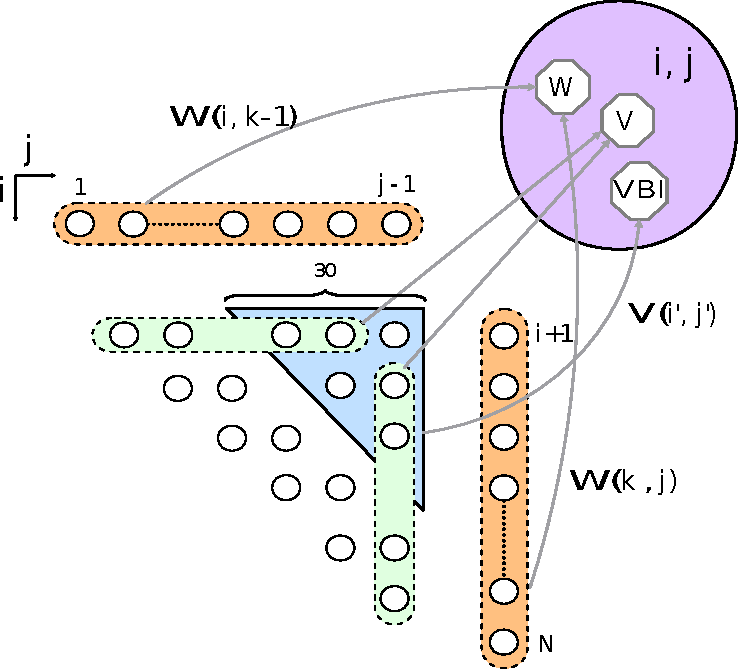
\includegraphics[width=8cm]{inc/zuker_rec.pdf}\end{center}
The recurrence consists of two non-serial dependencies as in \textit{\nameref{aswat}} plus a bounded 2-dimensional dependency for bulges.\\[12pt]
Since this problem is non-trivial to understand from the recurrences, we propose an additional illustration of a RNA chain folded according to the Zuker folding algorithm.
\begin{center}
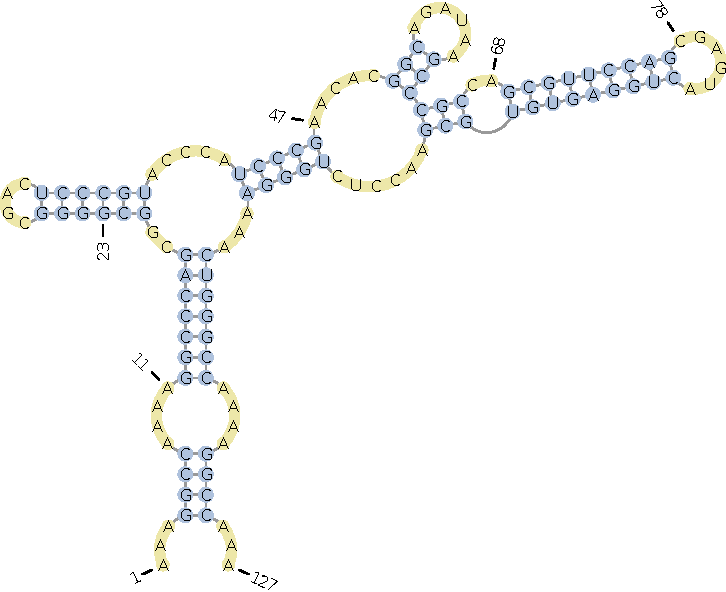
\includegraphics[width=10cm]{inc/zuker_struct.pdf} \\
\small An example of an RNA folded into a secondary structure. Types of structural features modeled by the Zuker folding algorithm include: dangling ends (1), internal loop (11), stack (23), multi-loop (47), bulge (68) and hairpin loop (78).
\end{center}

\item Optimizations: notice that there are 3 matrices: $W$,$V$ ($VBI$ is part of $V$) that can be expressed using regular matrix, and $F$ that is of different dimension than $W$ and $V$ and requires a special construction. Also notice that the $k$ of $BV$ and $BW$ describe almost the same backtrack, but there is an additional cost $c$ in $BV$.
%{\color{red} XXX: We need to find a nice way to encode both its construction and backtrack into the existing framework (implement 1D DP recursively?) }
\ole

% ------------------------------------------------------------------------------------------------
\newpage
\subsection{Related problems}
The goal of this section is to demonstrate that the problems described above are very similar or encompass a significant part of the common dynamic programming problems. (There is an hyperlink on the problems name to their detailed description).

\subsubsection{Serial problems}
\begin{tabular}{llcc} \toprule
\bf Problem & \bf Shape & \bf Matrices & \bf Wavefront \\ \midrule
Smith-Waterman \footnotesize simple & rectangle & 1 & -- \\
Smith-Waterman \footnotesize affine gap extension & rectangle & 3 & (can replace 2 matrices) \\
\href{http://en.wikipedia.org/wiki/Needleman-Wunsch_algorithm}{Needleman-Wunsch} & rectangle & 1 & -- \\

\href{http://en.wikipedia.org/wiki/Dynamic_programming#Checkerboard}{Checkerboard} & rectangle & 1 & -- \\
\href{http://en.wikipedia.org/wiki/Longest_common_subsequence_problem\#Code_for_the_dynamic_programming_solution}{Longest common subsequence} & rectangle & 1 & -- \\
\href{http://en.wikipedia.org/wiki/Longest_common_substring_problem\#Pseudocode}{Longest common substring} & triangle & 1 & -- \\
\href{http://en.wikipedia.org/wiki/Levenshtein_distance\#Computing_Levenshtein_distance}{Levenshtein distance} & rectangle & 1 & -- \\
\href{http://en.wikipedia.org/wiki/De_Boor's_algorithm}{De Boor} \footnotesize evaluating B-spline curves & rectangle & 1 & -- \\
\end{tabular}

\subsubsection{Non-serial problems}
\begin{tabular}{llcc} \toprule
\bf Problem & \bf Shape & \bf Matrices & \bf Wavefront \\ \midrule
Smith-Waterman \footnotesize arbitrary gap cost & rectangle & 1 & -- \\
Convex polygon triangulation & triangle & 1 & -- \\
Matrix chain multiplication & triangle & 1 & -- \\
Nussinov & triangle & 1 & -- \\
Zuker folding & triangle & 3 & -- \\
\href{http://en.wikipedia.org/wiki/CYK_algorithm}{CYK} \footnotesize Cocke-Younger-Kasami & triangle & \#rules & -- \\
\href{http://en.wikipedia.org/wiki/Knapsack_problem#Dynamic_programming}{Knapsack} \footnotesize (pseudo-polynomial) & rectangle & 1 & --\\
\end{tabular}

\subsubsection{Other problems}\ul
\item Dijkstra shortest path: we need a $E\times V$ matrix, along $E$ forall $V$ reduce its distance, problem is serial along $E$, non-serial along $V$ hence of complexity $O(|E|\cdot |V^2|)$ which is far worse than both $O(|V|^2)$ (min-priority queue) and $O(|E|+|V|\log |V|)$ (Fibonacci heap).
\item Fibonacci: this problem is serial 1D. Could be implemented using a placeholder element in one of the matrix dimension.
\item \href{http://archive.ite.journal.informs.org/Vol3No1/Sniedovich/\#dpmodel}{Tower of Hanoi}: 1D non-serial
\item \href{http://www.cs.ust.hk/mjg_lib/bibs/DPSu/DPSu.Files/KnPl81.PDF}{Knuth's word wrapping}: 1D non-serial
\item \href{http://en.wikipedia.org/wiki/Longest_increasing_subsequence#Efficient_algorithms}{Longest increasing subsequence}: serial (binary search is more efficient).
\item \href{http://www.ccs.neu.edu/home/jaa/CSG713.04F/Information/Handouts/dyn_prog.pdf}{Coin Change}: 1D non-serial
\ule

These algorithm also involve dynamic programming. However, we do not evaluate thoroughly their shape and number of matrices as this is not relevant in the scope of this project.\ul
\item \href{http://en.wikipedia.org/wiki/Floyd-Warshall_algorithm}{Floyd-Warshall}
\item \href{http://en.wikipedia.org/wiki/Viterbi_algorithm}{Viterbi \footnotesize (hidden Markov models)}: $T$ non-serial iterations over a vector
\item \href{http://en.wikipedia.org/wiki/Bellman-Ford_algorithm}{Bellman-Ford} (finding the shortest distance in a graph)
\item \href{http://en.wikipedia.org/wiki/Earley_parser#Pseudocode}{Earley parser} (a type of chart parser)
\item \href{http://en.wikipedia.org/wiki/Maximum_subarray_problem}{Kadane maximum subarray} 1D serial, look at 
\href{http://www.cosc.canterbury.ac.nz/tad.takaoka/cats02.pdf}{Takaoka} for 2D
\item \href{http://rna.tbi.univie.ac.at/cgi-bin/RNAfold.cgi}{RNA structure prediction}
\item \href{http://en.wikipedia.org/wiki/Recursive_least_squares_filter}{Recursive least squares}
\item \href{http://www.math.utep.edu/Faculty/pmdelgado2/courses/adv_algorithms/homework-08_anser.pdf}{Bitonic tour}
\item \href{http://www.cs.berkeley.edu/~vazirani/algorithms/chap6.pdf}{Shortest path, Shortest path in DAGs, All pair shortest paths, Independent sets in trees}
\item \href{http://www.algorithmist.com/index.php/Dynamic_Programming}{Subset Sum, Family Graph}
\item \href{http://www.cs.uiuc.edu/~jeffe/teaching/algorithms/notes/05-dynprog.pdf}{Optimal Binary Search Trees}
\item \href{http://www.cs.ucsb.edu/~suri/cs130b/NewDynProg.pdf}{Independent set on a tree}
\item \href{http://en.wikipedia.org/wiki/Dynamic_programming#A_type_of_balanced_0.E2.80.931_matrix}{More dynamic programming problems from Wikipedia}
\ule

\subsubsection{Conclusion}
In the rest of the project, we use a different description of the problems that is based on ADP \cite{adp}, which is more convenient but does not share much with the above description (even though ultimately the executed computations are very similar). Although not of immediate use, the description of the above problem and ad-hoc CUDA implementation of three of them (Smith-Waterman with arbitrary gap cost, Matrix chain multiplication and Convex polygon triangulation) helped us to understand:\ol
\item There is a difference between dynamic programming as seen in algorithmic classes and their concrete implementation, mainly because special care must be taken for correct indices and preventing off-by-one errors.
\item Problems can be classified in two categories: single track (input) and two-tracks (2 input sequences). Most of the common dynamic programming problems fall in these two categories.
\item Sometimes matrices are initially padded with zeroes (or initial value), although this might be ignored at algorithm design, care must be taken for these special values and their inclusion in the matrix should be decided according to the complexity of the recurrence formula.
\ole
